\subsection{Linearization}

The shallow water equation can be written in quasilinear form as \begin{align*}
u_t + f'(u) u_x = 0
\end{align*}
where $ u = (h,hv)^T $,
\begin{align*}
f'(u) = \begin{pmatrix}
0 & 1 \\
-(\frac{u_2}{u_1})^2 + gu_1 & 2 (\frac{u_2}{u_1})
\end{pmatrix}
\end{align*}
and 
\begin{align*}
q(x,0) &= \begin{pmatrix}
H + \epsilon e^{-(x-L/2)^2/w^2} \\
0
\end{pmatrix} 
\end{align*}
Now, to make this system linear we must simply pick a constant state $(h_0,v_0)$ which is consistent with the boundary and initial conditions. We choose $(h_0,v_0)$ at $x=0$ and $t=0$. We can now compute $(h_0,v_0)$ using the initial condition. We get $(h_0,v_0) \approx (1,0)$. Thus we have 
\begin{align*}
f'(u) = \begin{pmatrix}
0 & 1 \\
g & 0
\end{pmatrix} = \begin{pmatrix}
0 & 1 \\
9.61 & 0
\end{pmatrix}
\end{align*}
We can see easily $f'(u)$ has eigenvalues $\lambda_{1,2} = \pm \sqrt{9.61} = \pm 3.1$ which are real. It also has a full set of eigenvectors i.e. $(1,3.1)^T$ and $(-1,3.1)$. This together confirm that the linear problem is hyperbolic. We also know that the wave speeds are the eigenvalues, so we have wave speeds $\pm \sqrt{9.61}$

\subsubsection{Analytical Solution}
We have the PDE, 
\begin{align*}
q_t + f'(u) q_x = 0
\end{align*}
which we have shown can be written as 
\begin{align*}
q_t + V D V^{-1} q_x &= 0 \\
\implies V^{-1} q_t + D V^{-1} q_x &= 0
\end{align*}
where 
\begin{align*}
 V = \begin{pmatrix}
1 & -1 \\
3.1 & 3.1
\end{pmatrix}, \enspace D= \begin{pmatrix}
3.1 & 0 \\
0 & -3.1
\end{pmatrix},  \enspace \text{and} \enspace V^{-1} = \begin{pmatrix}
0.5 & 0.1613 \\
-0.5 & 0.1613
\end{pmatrix}
\end{align*} and initial condition
\begin{align*}
q(x,0) &= \begin{pmatrix}
H + \epsilon e^{-(x-L/2)^2/w^2} \\
0
\end{pmatrix}, \quad \quad 0 \leq x \leq L
\end{align*}
Now, defining a new variable $r = V^{-1} q$ we have the decoupled system of equations
\begin{align*}
r_t + Dr_x = 0
\end{align*}
and 
\begin{align*}
r(x,0) = V^{-1} q(x,0) = \frac{1}{2} \begin{pmatrix}
H + \epsilon e^{-(x-L/2)^2/w^2} \\
-H - \epsilon e^{-(x-L/2)^2/w^2}
\end{pmatrix} 
\end{align*}
From Lavengen, we know the solutions of this system are 
\begin{align*}
	r_1(x,t)&=r_1(x+\lambda_1t,0)=\frac{1}{2} (H + \epsilon e^{-(x+3.1t-L/2)^2/w^2}) \\
	\text{and} \quad r_2(x,t)&=r_2(x+\lambda_2t,0)= \frac{1}{2}(-H - \epsilon e^{-(x-3.1t-L/2)^2/w^2})
\end{align*} 
Finally switching back to $q$, we get 
\begin{align*}
q(x,t) = Vr(x,t) &= \frac{1}{2} \begin{pmatrix}
H + \epsilon e^{-(x+3.1t-L/2)^2/w^2} +H + \epsilon e^{-(x-3.1t-L/2)^2/w^2} \\
3.1(H + \epsilon e^{-(x+3.1t-L/2)^2/w^2} -H - \epsilon e^{-(x-3.1t-L/2)^2/w^2})
\end{pmatrix} \\
&= \frac{1}{2}\begin{pmatrix}
 2H + \epsilon e^{-(x+3.1t-L/2)^2/w^2} + \epsilon e^{-(x-3.1t-L/2)^2/w^2} \\
3.1( \epsilon e^{-(x+3.1t-L/2)^2/w^2} - \epsilon e^{-(x-3.1t-L/2)^2/w^2})
\end{pmatrix}
\end{align*} 
Now, simply plugging in $t=1$ we get
\begin{align*}
q(x,1) = \frac{1}{2}\begin{pmatrix}
 2H + \epsilon e^{-(x+3.1-L/2)^2/w^2} + \epsilon e^{-(x-3.1-L/2)^2/w^2} \\
3.1( \epsilon e^{-(x+3.1-L/2)^2/w^2} - \epsilon e^{-(x-3.1-L/2)^2/w^2})
\end{pmatrix}
\end{align*}
which is plotted in \ref{anal}.
We note that this solution does take into account any boundary conditions, and that the waves will not be reflected. However the waves have not hit the walls until after $T=1$ so our analytical solution still holds at $T=1$. 

\begin{figure}
\begin{center}
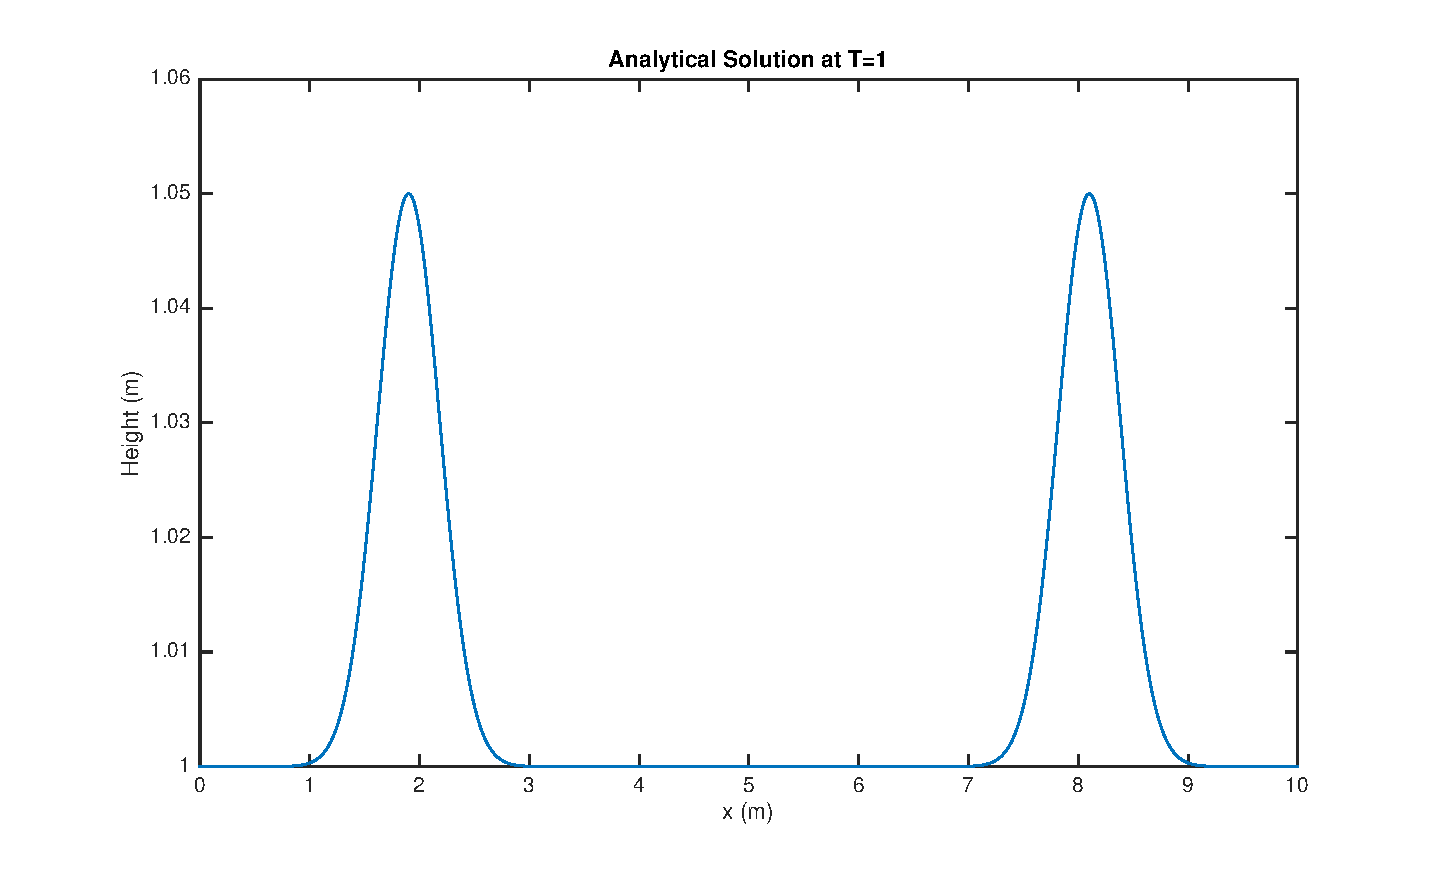
\includegraphics[scale=0.35]{analytical.eps}
\caption{Analytical Solution of the Linear Problem}
\label{anal}
\end{center}
\end{figure}

\subsubsection{Numerical Solution of the Linear Problem}
To compare the results from the non-linear and linear problems, we compare the numerical solutions of the problems using the same method and the proper boundary conditions. The code for the numerical solution of the linear problem is almost exactly the same as for the linear problem, except the flux $f$. For the linear problem we compute the flux function from the information above. 
\begin{align*}
f'(u) = \begin{pmatrix}
0 & 1 \\
g & 0
\end{pmatrix} \rightarrow 
f(u) = \begin{pmatrix}
u_2 \\
gu_1
\end{pmatrix}
\end{align*}
We plot the linear and non-linear numerical solutions in \ref{compare} so they can be compared on the same plots. 
\begin{figure}
\begin{center}
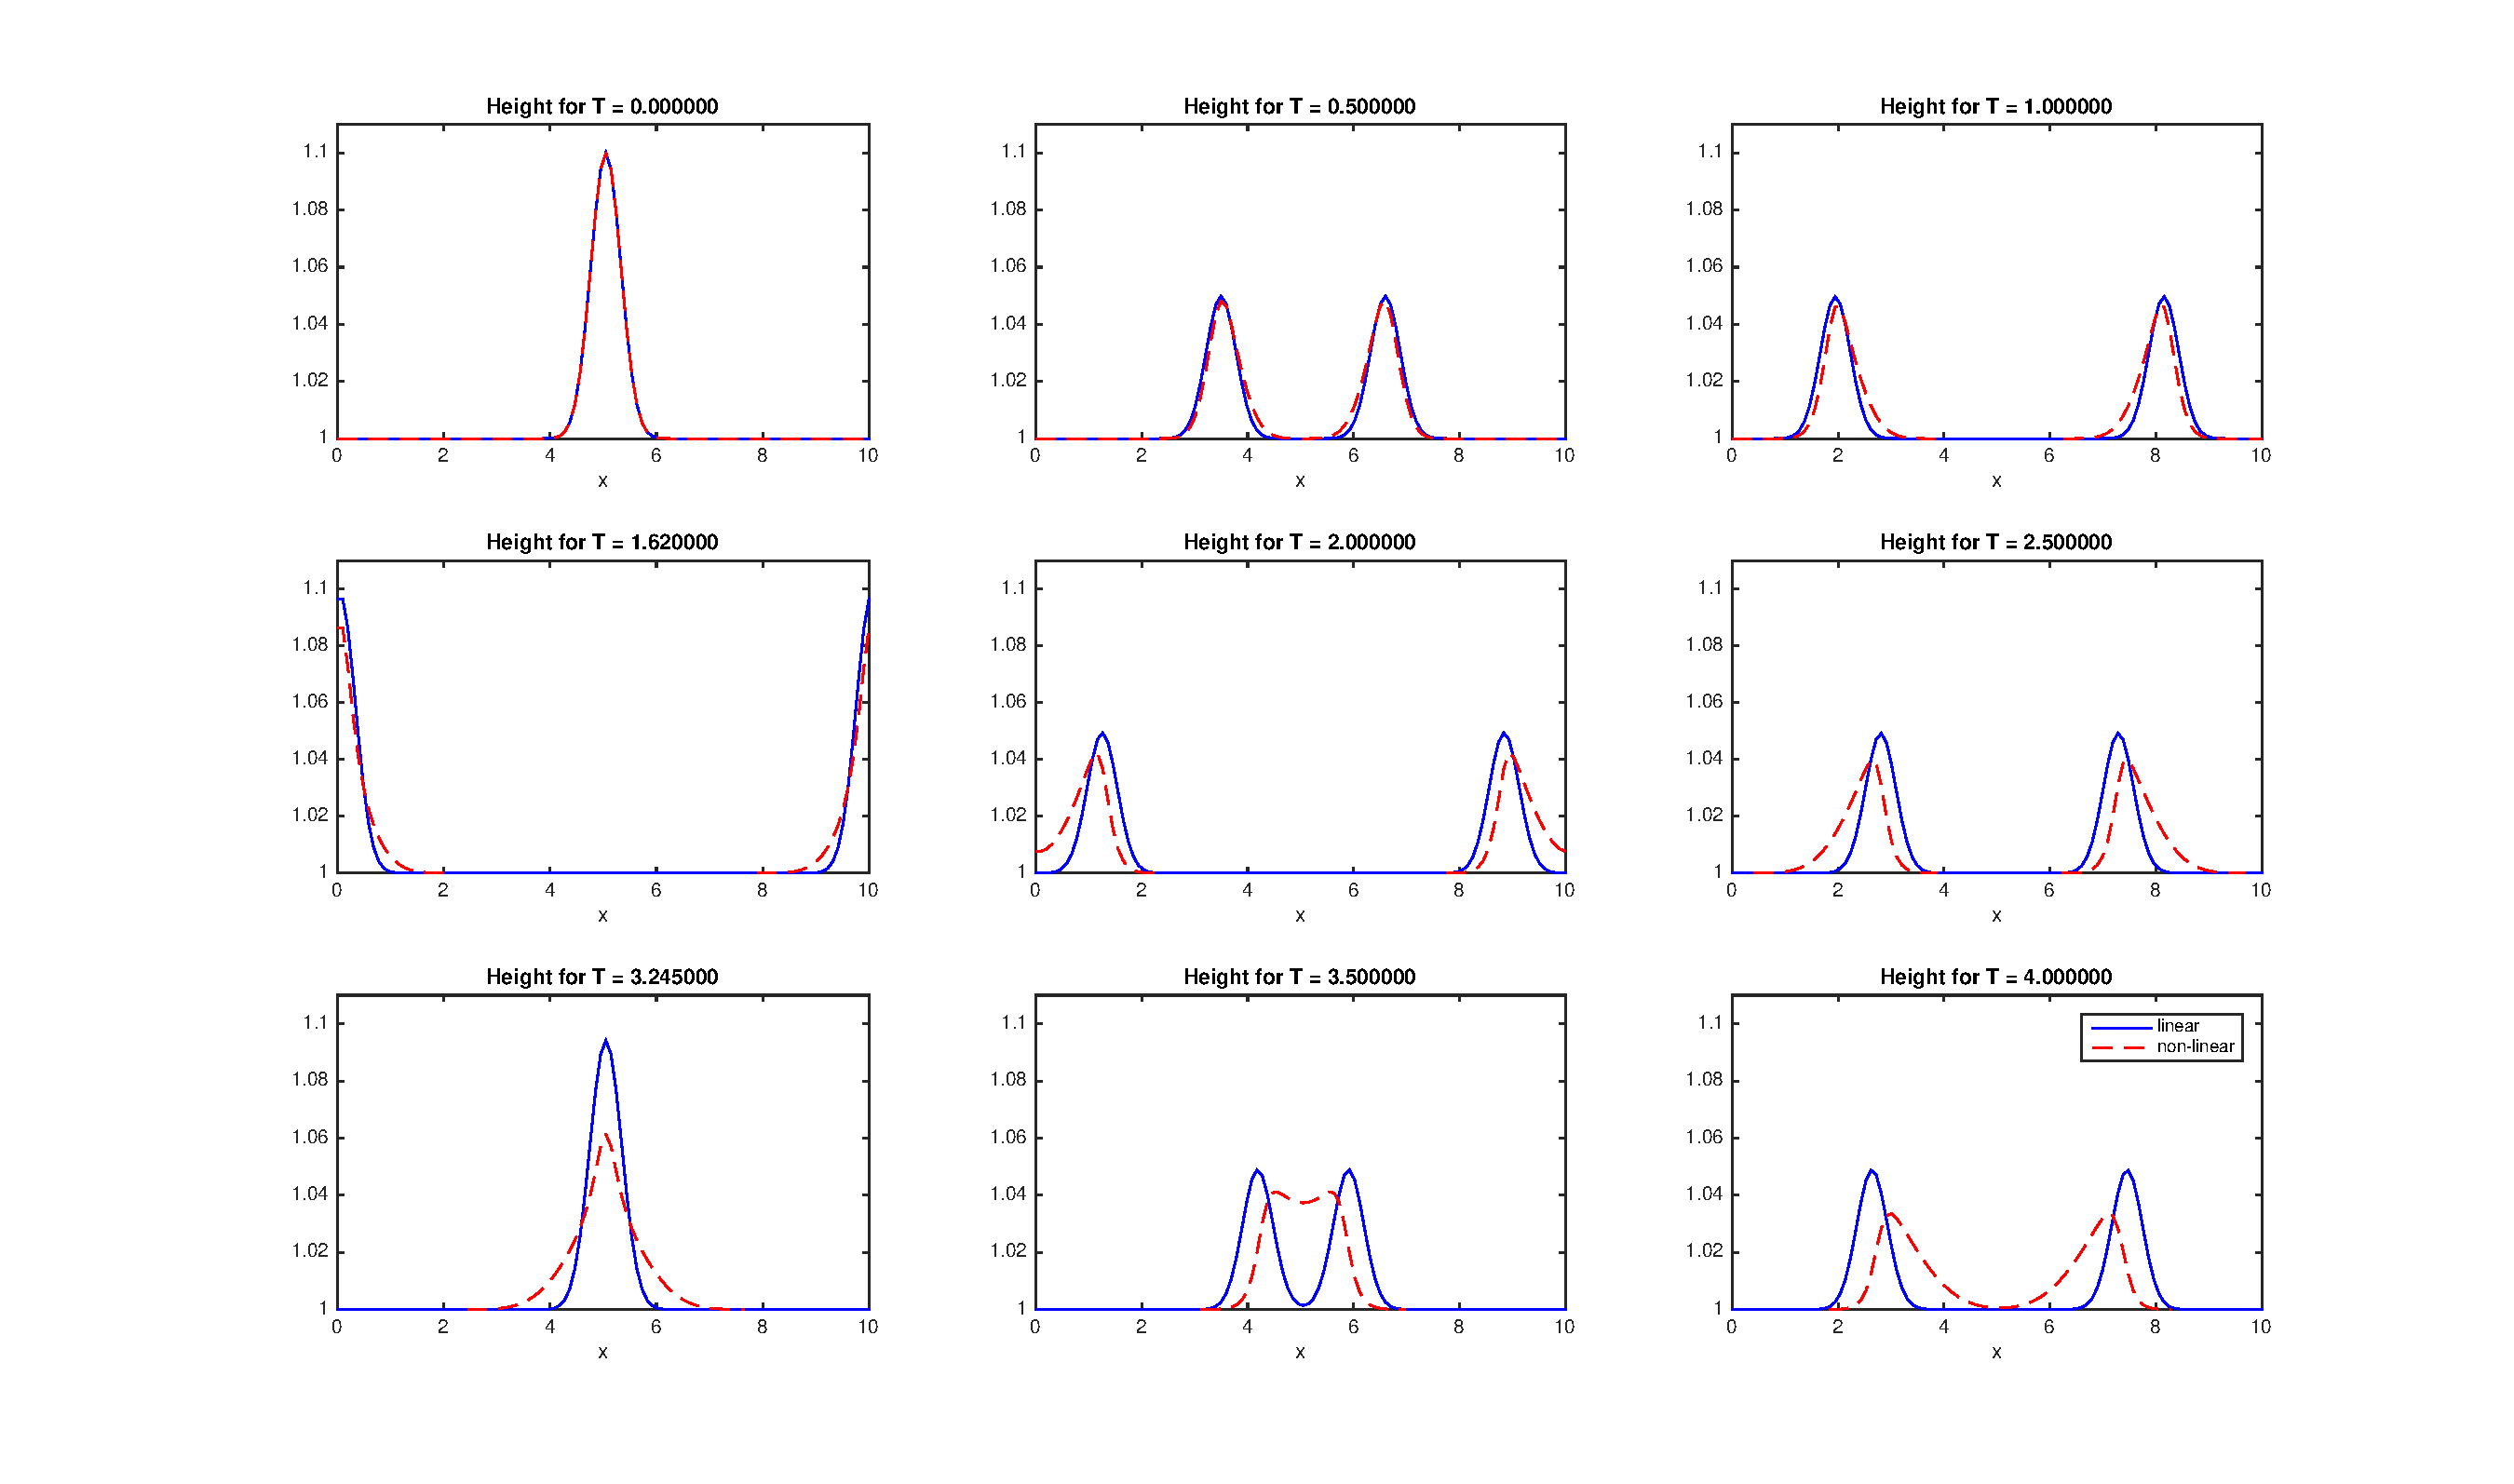
\includegraphics[scale=0.35]{222comparison.eps}
\caption{Comparison of Linear and Non-linear Problems}
\label{compare}
\end{center}
\end{figure}
The first thing we can see is that the waves from the linear solution are totally symmetrical. This is in contrast to the non-linear problem, in which the waves are already noticeably unsymmetrical at $T=1$. The second difference that we notice is that the waves in the linear case retain their shape (same width and height) before and after collisions. In the non-linear case, this is not true. One can see that after a collision, the waves in the non-linear solution become shorter and wider. We can also see that the linear waves move quicker than the non-linear waves. 